\subsubsection{Caso d’uso UC8.2.1.5: Modifica domanda a ordinamento di immagini}
\label{UC8.2.1.5}
	\begin{figure}[h]
		\centering
			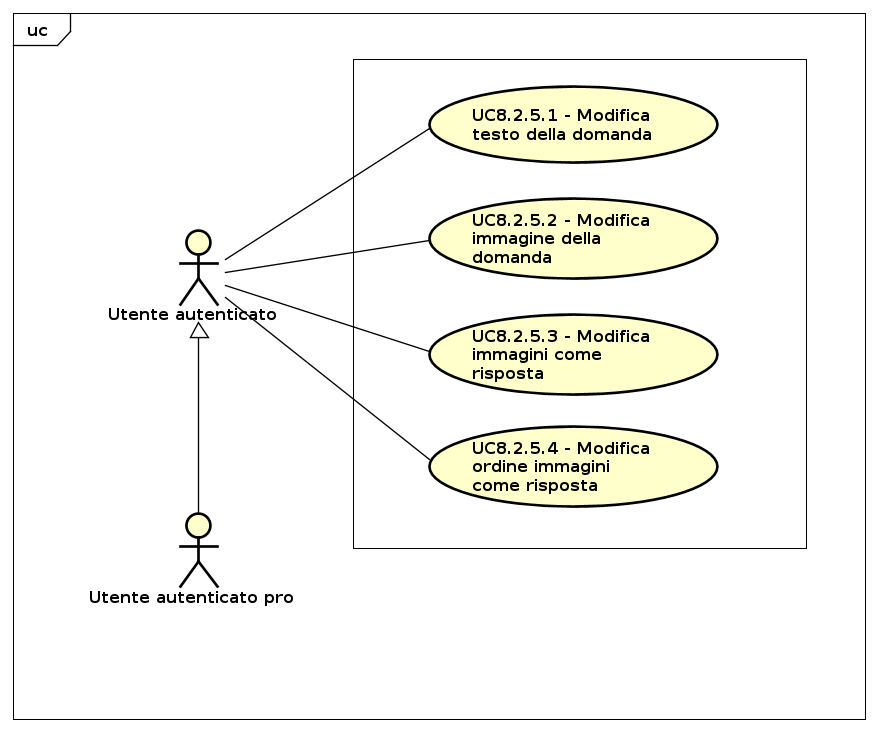
\includegraphics[scale=0.45,keepaspectratio]{UML/UC8_2_1_5.png}
		\caption{UC8.2.1.5: Modifica domanda a ordinamento immagini}
	\end{figure}
\begin{itemize}
	\item\textbf{Attori}: utente autenticato, utente autenticato pro;
	\item\textbf{Scopo e descrizione}: gli attori possono modificare una domanda del tipo ordinamento di immagini;
	\item\textbf{Precondizione}: il sistema mostra agli attori il form di modifica dei campi dati per la tipologia di domanda scelta; 
	\item \textbf{Postcondizione}: gli attori hanno inserito tutti i campi dati obbligatori;
	\item\textbf{Scenario principale}: 
	\begin{itemize}
		\item Gli attori possono modificare il testo della domanda (UC8.2.1.5.1);
		\item Gli attori possono modifica l'immagine allegata al testo della domanda (UC8.2.1.5.2);
		\item Gli attori possono modificare le immagini relative alla risposta (UC8.2.1.5.3);
		\item Gli attori possono modifica l'ordine corretto delle immagini relative alla risposta (UC8.2.1.5.4);
	\end{itemize}
\end{itemize}

\subsubsection{Caso d’uso UC8.2.1.5.1: Modifica del testo della domanda}
\begin{itemize}
	\item\textbf{Attori}: utente autenticato, utente autenticato pro;
	\item\textbf{Scopo e descrizione}: gli attori possono modificare il testo della domanda;
	\item\textbf{Precondizione}: il sistema mostra agli attori il form di modifica del testo della domanda; 
	\item \textbf{Postcondizione}: gli attori hanno inserito il nuovo testo della domanda;
	\item\textbf{Scenario principale}: gli attori possono modificare il testo della domanda;
\end{itemize}

\subsubsection{Caso d’uso UC8.2.1.5.2: Modifica dell'immagine della domanda}
\begin{itemize}
	\item\textbf{Attori}: utente autenticato, utente autenticato pro;
	\item\textbf{Scopo e descrizione}: gli attori possono modificare l'immagine allegata alla domanda;
	\item\textbf{Precondizione}: il sistema mostra agli attori il form di modifica dell'immagine della domanda; 
	\item \textbf{Postcondizione}: gli attori hanno inserito la nuova immagine allegata alla domanda;
	\item\textbf{Scenario principale}: gli attori possono modificare l'immagine allegata alla domanda;
\end{itemize}

\subsubsection{Caso d’uso UC8.2.1.5.3: Modifica delle immagini della risposta}
\begin{itemize}
	\item\textbf{Attori}: utente autenticato, utente autenticato pro;
	\item\textbf{Scopo e descrizione}: gli attori possono modificare le immagini relative alla risposta;
	\item\textbf{Precondizione}: il sistema mostra agli attori il form di modifica delle immagini relative alla risposta; 
	\item \textbf{Postcondizione}: gli attori hanno inserito le nuove immagini relative alla risposta;
	\item\textbf{Scenario principale}: gli attori possono modificare le immagini della risposta;
\end{itemize}

\subsubsection{Caso d’uso UC8.2.1.5.4: Modifica ordine immagini della risposta}
\begin{itemize}
	\item\textbf{Attori}: utente autenticato, utente autenticato pro;
	\item\textbf{Scopo e descrizione}: gli attori possono modificare l'ordine corretto delle immagini relative alla risposta;
	\item\textbf{Precondizione}: il sistema mostra agli attori il form di modifica dell'ordine delle immagini relative alla risposta; 
	\item \textbf{Postcondizione}: gli attori hanno inserito il nuovo ordine delle immagini relative alla risposta;
	\item\textbf{Scenario principale}: gli attori possono modificare l'ordine dele immagini relative alla risposta;
\end{itemize}